\documentclass[twocolumn]{ctexart}
\usepackage{fancyhdr}
\pagestyle{empty}
\usepackage{graphicx}
\usepackage{geometry}
\geometry{
  margin=0cm,
  left=1cm,
  right=1cm,
  headheight=0cm,
  headsep=0cm,
  top=1cm,
  bottom=1cm,
}
\setlength\parindent{0cm}
\renewcommand{\emph}[1]{\textbf{\underline{#1}}}
\begin{document}
\zihao{-6}
\fbox{信息网络概述}
\emph{为什么需要交换}减少网络中节点之间所需的通信线路,增强可扩展性,构建更大规模网络
\emph{交换操作的过程}为输入数据选择输出线路/端口,在输入和输出之间建立连接,通过该连接将数据放到输出线路/端口上
\emph{电路交换}交换传输线路(空分交换)或者时隙(时分交换),通过交换机在通信双方之间建立一条专用的传输路径,或者占用传输线路的某一个固定的时隙,数据像流一样在路径上传输
\emph{电路交换特点}优点:占用固定线路资源,保证数据传输的速率、延时、可靠性、有序性;缺点:线路资源利用率低,没有数据传输时也占用线路或固定时隙,电路连接导致延迟;为话音传输设计,支持固定的数据速率
\emph{分组交换IP}交换分组,以分组为单元统计复用线路(链路)资源
\emph{统计复用}只有有数据要传输才占用线路
\emph{分组大小}太小则开销大;太大则复用效率低,影响其他分组发送
\emph{分组交换特点}优点:线路利用率高,节点只有在有数据数据要传输才占用线路,因此多个节点的分组可以共享一条通信线路;
缺点:需要资源管理机制来保证数据传输的速率、延时、可靠性和有序性,增加了复杂性;
以分组为单位统计复用线路/链路资源;
为数据传输设计,支持可变数据传输速率
\emph{数据报}直接发送分组
\emph{数据报特点}无连接,无QoS;
健壮性,分组携带的控制信息有目的地址,相同源目的的分组可能沿不同路径传输可绕开故障路径,交换机根据路由表独立转发分组
\emph{虚电路ATM}先建立连接再发送分组
\emph{虚电路特点}面向连接:与电路交换不同,连接不占用固定资源,只是告诉网络资源需求,在交换机上建立连接状态,有QoS;
有有序性,同一源目的的分组沿相同路径到达目的;
基于虚电路标识VCI执行交换操作,速率高
\emph{现有网络体系结构}OSI七层模型(物理层、数据链路层、网络层、传输层、会话层、表示层、应用层);Internet体系结构(基于TCP/IP参考模型,网络接口层、互联网层、传输层、应用层)
\emph{当前网络问题}端到端路径不存在:DTN路由(Delay Tolerant Network,时延容忍网络),引入Bundle Protocol(可在TCP/IP和非TCP/IP中运行)。
缺乏控制机制:SDN(Software Defined Networking,软件定义网络),基本思想是数据面与控制面分离。
可扩展性、移动性、服务质量、网络安全、能耗:FIA(Future Internet Architecture,未来网络架构)
FIA冗余传输问题:NDN(Named Data Networking,内容命名网络),通过自动缓存优化带宽,确保内容安全。
IP地址问题:MobilityFirst,路由器缓存减少数据丢失

\fbox{接入网技术}
\emph{网络拓扑}Ad Hoc网络(自组织网络):STA(无线站点)之间通过无线传输媒介组成网络;基础设施网络,STA间通信必须通过AP(无线接入点,网络名SSID,STA配置必须与AP相同)
\emph{CSMA/CA}带冲突避免的载波侦听多路访问机制:
载波侦听 :站点在发送帧之前侦听无线信道是否空闲,如果是,则进入冲突避免阶段,如果当前信道忙,说明现在有其它站点正在传输数据,则延迟发送帧直到侦听到信道空闲;
– 冲突避免:站点在发送帧之前要先等待一个帧间间隔IFS,并且确保在 IFS 时间内信道空闲;
为了防止多个站点在等待 IFS 时间后同时发送而导致冲突,与以太网类似,引入了一个随机退避算法来选择一个退避时间
\emph{CSMA/CA流程}侦听信道闲(忙则一直侦听)—等待IFS(InterFrame Spacing,帧间隔)—信道闲—(随机退避避免同时发送)—发送
\emph{为何不使用CSMA/CD}在以太网中,同一网段内任何数据传输数据其它的主机都能侦听到,无线环境下无线信号覆盖范围有限,信道之间的冲突很难让其它设备检测到
\emph{扩展CSMA/CA}发送方发送 RTS 帧,其中包含了一个持续时间域,该域的值表明发送方完成帧交换所需要的时间,包括从发送数据帧到接收 ACK 帧所需要的时间;
收到 RTS 的站点根据其中的持续时间为自己声明一个虚拟信道,并且该信道正忙,用网络分配向量(NAV)来表示,在 NAV 时间内,该站点不会尝试发送帧;
接收方响应 CTS 帧中也包含一个持续时间域,该域的值足够大,以保证发送方能够完成数据帧交换;
收到 CTS 的站点根据其中的持续时间为自己声明一个虚拟信道,并且该信道正忙;
NAV 更新:只有当RTS/CTS中的持续时间域的值大于当前存储的NAV时,该NAV才会被更新
\emph{扩展CSMA/CA解决问题}隐藏站点、暴露站点
\emph{光接入网Optical Access Network}采用光纤传输技术,提供 Gbps 量级的宽带接入,支持传统电话、电视,以及数据等综合业务
\emph{无源光网络Passive Optical Network}接入路径上使用无源的光分/合路器,不进行光电转换;
多个用户共享光纤,性价比高
\emph{关键问题}如何控制多个ONU/ONT对共享馈线光纤的高效访问
\emph{关键技术}下行数据安全性:采用广播方式传输,需要对数据进行加密;
上行数据发送冲突问题,采用TDMA同步:主/从模式:ONU/ONT请求,OLT授权ONU/ONT 访问指定时隙(下行不需要MAC,上行需要MAC 控制对共享光纤的访问);测距(Ranging):ONU/ONT到OLT的距离为0--20km ,传输延迟不同(0--200us) ,环境变化也会对传输延迟差生影响,通过测距给ONT/ONU插入延迟,确保其到 OLT 的逻辑距离一样;
动态带宽分配(DBA:DynamicBandwidth Allocation):OLT 通过动态分配共享光纤的传输时隙来提高带宽使用率,保证多业务服务质量

\fbox{IPv6协议}
\emph{IPv6 v.s. IPv4}32到128位,扩展地址空间;简化头标,提高路由器处理效率
\emph{路由表配置}无类别域间寻路CIDR采用可变长度的网络前缀(networkprefix)来取代地址分类中网络号长度固定的做法,具有相同前缀的 IP 地址组成 CIDR Block(A.B.C.D/N)N为前缀长度;
前缀汇聚:每个CIDR Block分配给一个网络,到该网络的路由通过CIDR Block前缀来标识;
多个连续的CIDR Block对应的网络如果连接在路由器的同一个端口下面,则在路由器上,到这些网络的路由可以用一个更短前缀来标识,该前缀对应的CIDR Block包含这些连续的CIDR Block
前缀最长匹配规则:在 CIDR 中,如果路由器上的路由表中有多条表项满足要求,则采用前缀最长
\emph{不需要全局地址}有些机制所需的信息在子网范围内都可以获得
\emph{单播地址}链路局部地址作用范围为链路,在链路范围内进行分配,由FE80::/64和64位接口ID组成;
全局地址(GUA):001和3--48位全局路由前缀组成站点前缀,48--64位为子网ID,后64位为主机接口ID
\emph{组播地址}形式(FF::/8),后4位为flag,指示组播地址是否是永久的;再后4位为Scope,指示范围(链路范围Scope=2),后跟112bits的组播组范围;
全节点地址FF02::1(链路范围);
全路由器节点地址FF02::2;
被请求节点地址(不知道接收方的MAC地址时)将前98位换为FF02::1:FF,保留24bits。组播地址在节点不知道其他节点或者网络任何信息时可以用组播地址通信。
\emph{IPv6邻居发现机制}
地址解析,用于IP分组转发过程,首先查找路由表得到下一跳IP地址。通过该IP地址解析得到MAC地址,并将其置为MAC帧的目的MAC地址。
地址解析通过邻居请求(Neighbor Solication,NS,其目的地址为被请求节点地址)和邻居公告(NA,Neighbour Advertisement)完成。首先判断是否需要解析(查找邻居缓存),如需要,则组播NS,包含需要解析的IPv6地址;目标节点响应NA,单播返回MAC地址,发送节点更新该地址。
地址重复检测DAD:防止全局地址重复。基于NS/NA,发送包含待测IPv6地址的NS,若收到NA则重复,不再使用该地址。
路由器发现:节点通过路由器发现过程找到本地链路上路由器的集合,获得所连接网络的信息,通过路由器公告(RA,Router Advertisement)和路由器请求(RS,Router Solicitation)实现,
配置其它网络参数:确定节点地址自动配置方式:是否使用有状态地址自动配置(DHCPv6);
为链路定义的网络前缀列表,每个前缀包含IPv6网络前缀和有效、推荐生存期;
IPv6头标中Hop limit 域的缺省设置;
本地链路的MTU
被动(IPv6路由周期性公告路由器公告RA消息,组播发送,统一链路上的IPv6主机接受RA消息并且使用其内容来配置或者维护网络参数设置,使用FF02::1);
主动(IPv6 主机主动发送路由器请求 RS组播发送,同一链路上的路由器响应RA,单播或组播方式发送,RS使用FF02::2)。
\emph{被请求节点地址作用}便于链路寻址,获得MAC地址;
NS的目的地址;
实现对主机的分组拦截
\emph{无状态地址自动配置}不通过额外的服务器来管理地址,不易于地址管理;有状态地址自动配置由DHCPv6服务器对地址进行统一分配和管理。
\emph{EUI-64地址}一种新的网络接口地址标准;
为网络设备制造商提供了更多地址空间;
与MAC地址互相映射;
24bit统一分配,第7位U/L确定是全局还是本地;第八位I/G确定是单播还是组播,一般均为0。可提供更多地址空间。在48位MAC地址的company ID与extension ID间(24位处)插入0xFFFE可实现二者转换。到IPv6地址则反转U。二者结合可实现MAC到IPv6的转换。
\emph{自动配置过程}链路局部地址:
基于FE80::/64 和 EUI-64地址生成的接口标识生成链路局部地址,设置为尝试(Tentative)状态;
执行地址重复检测(DAD)过程;
若DAD成功,将其设置为有效(Valid/Preferred)状态;
将链路局部地址的被请求节点地址所对应的组播MAC加到网络接口的感兴趣MAC地址表中。
对于IPv6主机,还将继续以下的全局地址自动配置过程。
路由器发现过程:主机发送路由器请求(RS)消息,路由器响应路由器公告(RA)消息,RA中包含网络前缀、缺省路由器、hop limit、MTU等信息;
根据网络前缀信息,开始地址自动配置过程:根据前缀和接口标识自动生成地址,设置为尝试(Tentative)状态;
对地址进行DAD过程;
如果DAD成功,设置地址状态为有效状态(Valid),根据前缀信息中的Valid Lifetime和Preferred Lifetime域来设置valid和preferred lifetime;
将配置地址的被请求节点地址所对应的组播MAC加到网络接口的感兴趣MAC地址表中。
根据RA中包含的其它信息进行缺省路由等网络参数的配置
\emph{手动配置隧道}对每个IPv6分组都事先手工配置它所对应的隧道的端点(用于隧道封装所需的IPv4地址)并配置到隧道的路由
\emph{自动配置}建立一个IPv6地址到IPv4地址之间的映射关系,分组中所包含的IPv6地址和路由器的下一跳决定隧道的端口(用于隧道封装所需的IPv4地址)并配置到隧道的路由
\emph{ISATAP地址}私有:64-bitUnicastPrefix:0:5EFE:w.x.y.z;全局:64-bitUnicastPrefix:200:5EFE:w.x.y.z;
64-bitUnicastPrefix可以为链路局部、全局和唯一本地前缀
\emph{6to4地址格式}:2002+32位全局IPv4地址+16位子网编号+64位主机ID

\fbox{IP网络移动管理}
\emph{切换}移动节点从一个接入点到另一个接入点的过程
\emph{五元组}标识应用会话,结构为源/目的IP地址、协议、源/目的端口号
\emph{类型}同一网络中不同AP的切换是链路层切换(不改变IP地址,五元组不变,对应用会话无影响);
不同网络不同AP之间首先执行链路层切换,再使用网络层切换,进行网络相关参数配置,IP地址变化导致会话中断。
\emph{问题}通信对端不知道移动节点地址发生变化,即使通信对端知道了地址二,由于五元组发生变化,会话也会中断。
\emph{方案}应用层需要应用支持,本质上是重新建立IP会话。网络层解决方案:需要增强网络协议,对应用透明
\emph{移动IPv6}移动节点检测到自己移动到外地网络,则发布RA;家乡代理更新家乡地址HoA与转交地址CoA的绑定缓存。当通信对端不支持IPv6时,采用双向隧道技术;支持时,采用路由优化模式,在通信对端修改绑定缓存。
\emph{实体}HoA:家乡地址;CNA:通信对端的地址;CoA:转交地址HAO:家乡地址选项,信宿选项头标;T2R:类型2寻路头标。
\emph{移动性屏蔽原理}对于IP层以上的应用来说,看到的始终是节点的家乡地址。
双向隧道模式下,移动节点和通信对端的通信始终使用家乡地址进行通信;移动节点的移动由家乡代理跟踪,对于通信对端来说是透明的;所有的通信都必须通过家乡代理转发。(通信对端向家乡代理发送目的为HoA,源为CN的包,家乡代理通过拦截技术进行拦截并封装,在IPv6-in-IPv6隧道中传输,外层包头源为家乡代理地址,目的地址为CoA。)
路由优化模式下通信对端知道移动节点当前的转交地址。移动节点收到包,绑定更新列表并添加通信对端,二者直接进行通信。
\emph{PMIPv6}代理移动IPv6,基于网络端的本地移动管理
\emph{为何引入}易于部署、管理、性能更好
\emph{原理}网络端控制的移动管理,移动接入网关:在网络中引入一个功能实体代理移动节点执行与家乡代理之间的信令;
本地移动管理,本地移动锚定点:在本地管理域中引入一个类似家乡代理的功能实体,负责管理域内的移动管理操作;
移动管理相关信令运行在移动接入网关和本地移动锚定点之间

\fbox{路由和交换}
\emph{路由器功能}数据路径功能:根据分组目的IP地址查找转发表,通过交换结构转发到输出端口,输出端口调度和队列管理;
控制面功能:运行路由协议,构建路由表,系统配置和管理。
\emph{交换与路由的区别}路由更宏观,是将分组从网络中的一个网络投递到另一个网络的过程:
需要网络中节点协作;
运行路由协议。
交换是指在同一个网络节点内的分组传输,指将分组从一个端口(输入端口)转发到另一个端口(输出端口)的过程:
属于网络设备自己的功能:
基于转发表,查找算法和交换结构
\emph{交换机与路由器的区别}交换机用于网络内互联,路由器用于不同网络互联
\emph{性能}查找速度:决定链路带宽( 10Gbps 链路要求每秒转发 31.25*106 个分组,最小 IP 分组长度为 40 字节)。
存储(空间)需求:存储访问速度、功耗;基于缓存的软件算法。
更新代价:在峰值时, Internet 上每秒钟的 BGP 路由更新有几百次,要求能够处理每秒上千次更新。
可扩展性:转发表预计每年都在增加。
实现的灵活性:既能软件实现,也能硬件实现。
\emph{Binary Trie}使用二进制Trie存储。问题:存在回溯操作
\emph{Leaf pushing}优化节点上的每个条目要么包含一个指针,要么包含下一跳信息,相当于把下一跳信息Push down到叶子节点
\emph{特点}增加更新复杂度,存储空间减少为1/2
\emph{Path Compression Trie}压缩只有一个子节点的非前缀节点
\emph{性能}路径压缩可以有效地减少稀疏 binary trie 的高度;在最差情况下,如果为完全树时,没有压缩的可能,因此采用路径压缩后查询和更新复杂度与 binary trie 一样,都是 O(W)
\emph{Multi-bit Trie}查找时同时检查多个比特,称为查找步长(Stride)。如果前缀长度不为步长的整数倍,则对其进行扩充。例如步长为3,对于前缀1*可以扩充为100,101,110,111步长为k,则Trie中的每个节点的条目数量为2k。每个条目组成:<下一跳信息,指向下一个子节点的指针(可以为空)>
\emph{性能}步长为 k 比特,则查找的复杂度为$O(W/k)$,W 为地址的长度;
更新复杂度$O(W/k2^k)$每个节点有 2k 个条目;
存储(空间)复杂度$O(N2^kW/k)$
\emph{LC Trie}在最差情况下, LC-Trie 的性能与步长为 k 的 Multi-bit Trie 差不多,但是由于使用了 Path Compression ,在实际情况下 LC-Trie 能够更加有效地利用存储空间
\emph{三代交换结构}共享存储器交换,速率受访问速度限制;
共享媒介交换,受限于总线速率;
空分交换,受限于交换结构
\emph{为何采用交换结构的高性能路由器的输出竞争不可避免}多个输入端口请求同一个输出端口导致输出竞争,由 IP 业务的突发性导致故不可避免
\emph{如何缓解输出竞争带来的问题}使用输出缓存即输出队列解决输出端口竞争

\fbox{网址}\textbf{MAC} IPv6 Prefix + MAC(前L/U):FF:FE:MAC(后)

例如2002:1:0:3:BEAE:C5FF:FEC2:721

\emph{全局ISATAP} IPv6 Prefix + :200:5EFE: + IPv4,例如2002:1::1:200:5EFE:160.0.0.2

\emph{局部ISATAP} FE80::200:5EFE: + IPv4,例如FE80::200:5EFE:160.0.0.2

\emph{Router} IPv6 Prefix on link; other routers;::/0 relay

\emph{Host} IPv6 Prefix on link; ::/0 router

\emph{6to4 Prefix} 2002:IPv4:SubnetID/64,例如2002:9D3C:1:1::/64

\emph{6to4 IP} 例如2002:9D3C:1:1::1

\emph{Router} 2002::/16 on link; other routers;::/0 relay

\emph{Host} IPv6 Prefix on link; ::/0 router

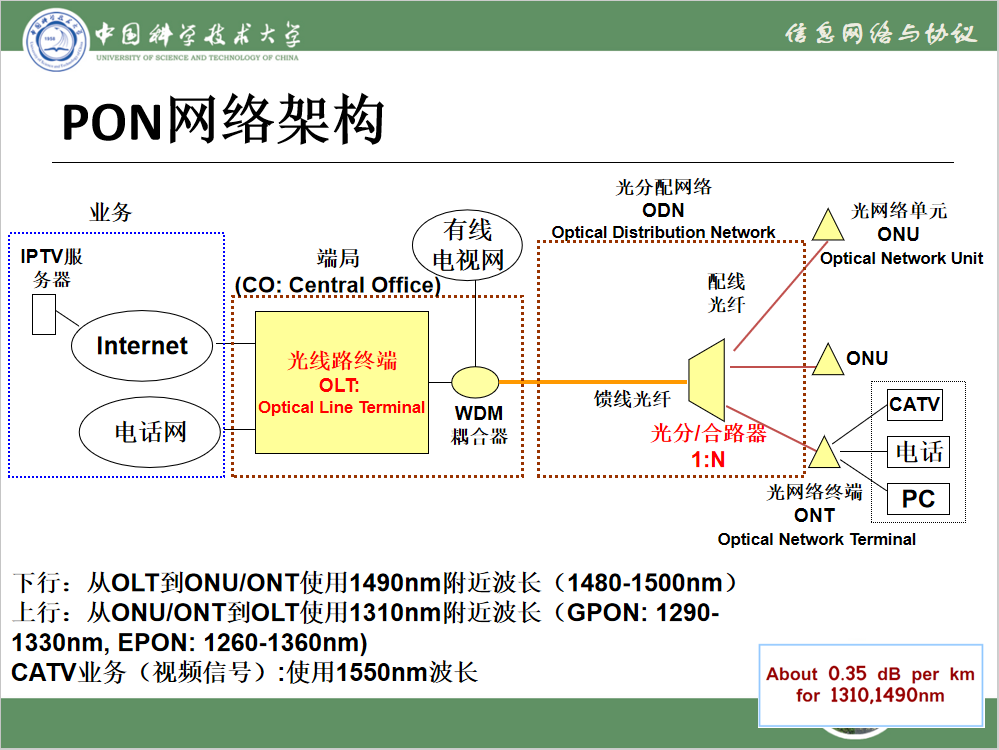
\includegraphics[
  width=\linewidth,
]{images/pon.png}

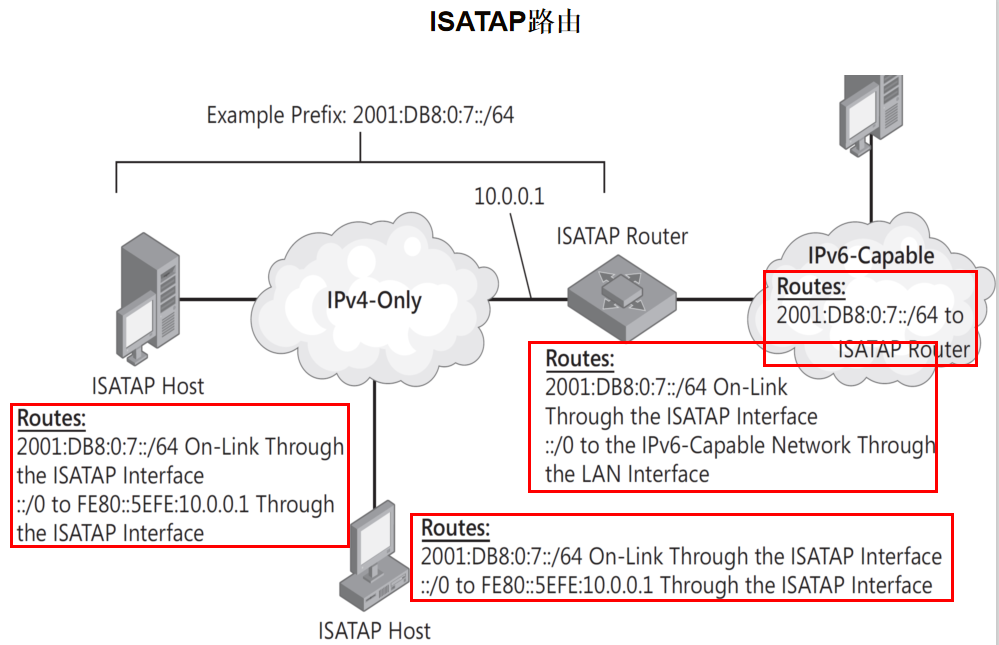
\includegraphics[
  width=\linewidth,
]{images/isatap.png}

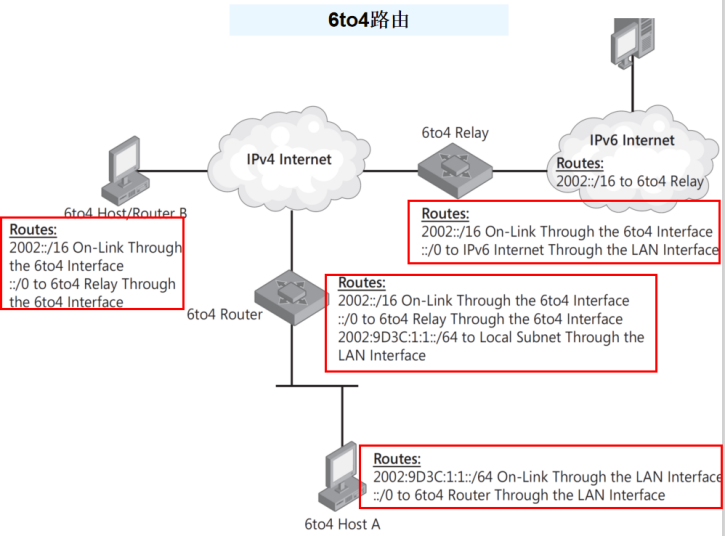
\includegraphics[
  width=\linewidth,
]{images/6to4.png}

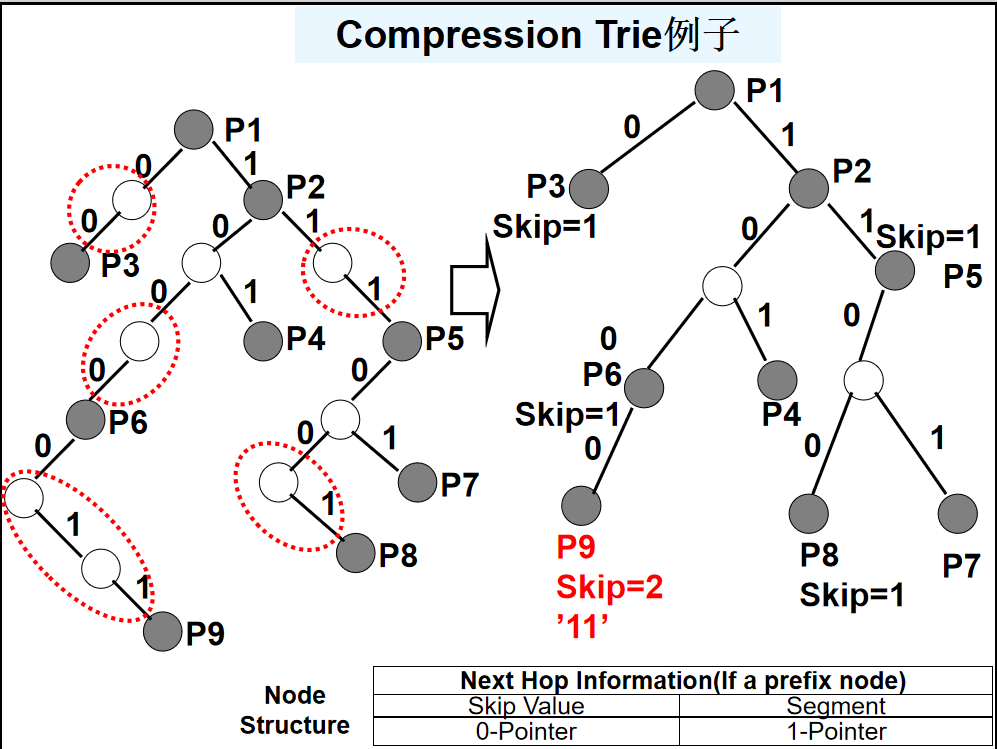
\includegraphics[
  width=\linewidth,
]{images/compression.png}

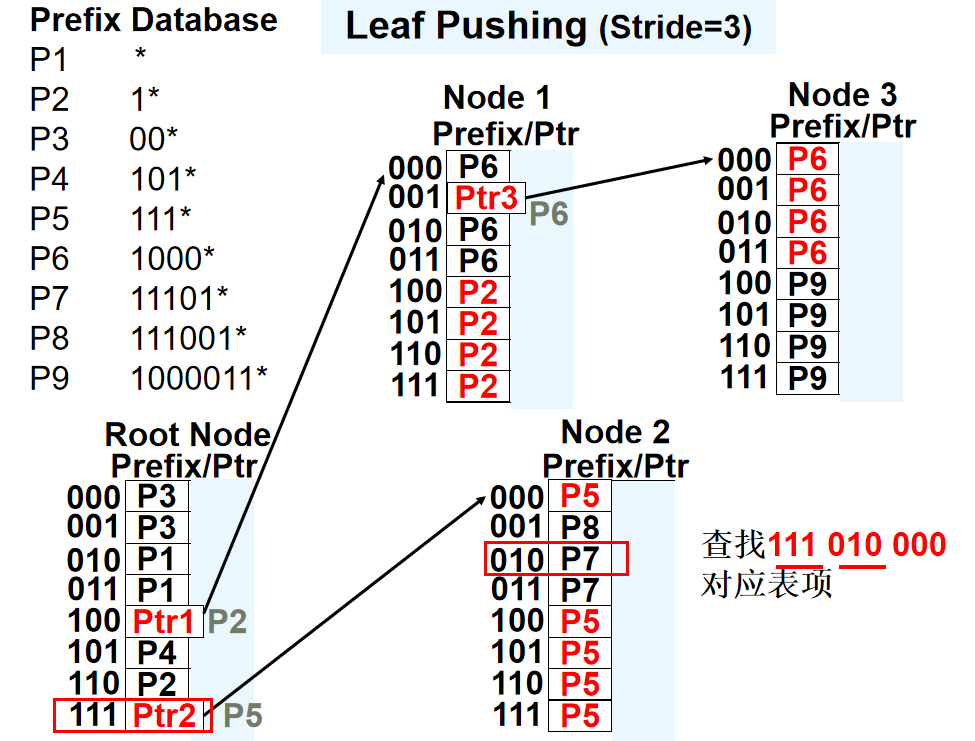
\includegraphics[
  width=\linewidth,
]{images/leaf.png}
\end{document}
